\begin{figure}[h]
    \centering
    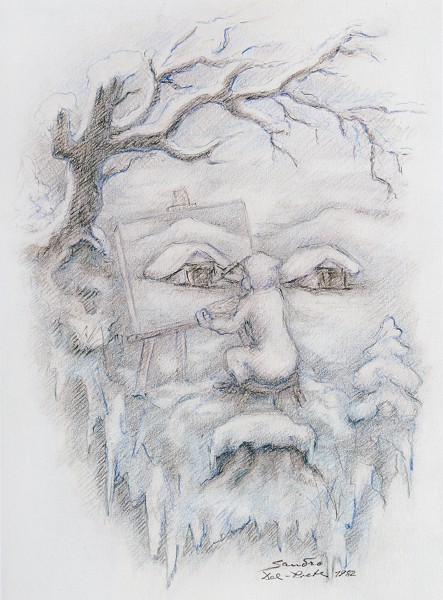
\includegraphics[width=0.8\textwidth]{sdp_mountain_spirit.jpg}
    \caption[Mountain Spirit in Winter by Sandro del Prete]{Mountain Spirit in Winter by Sandro del Prete. The image is from \citeay{sdp_mountain}.}
    \figlbl{sdp_mountain}
\end{figure}

One of the insights from the \emph{Gestalt} psychology \sidecite{ellis_source_1938, kohler_gestalt_1992, wagemans_century_2012, hamlyn_psychology_2017} is that humans are apparently able to recognize the Gestalt of an object within a very short time; The brain can immediately recognize global patterns - arrays of local features that consistently conform to a known large-scale pattern - even if those local features are buried in noise or would, on the basis of local context, be interpreted very differently. Thus, local decisions are made based on plausibility considering overall patterns, while the overall patterns can only be defined based on local features.

For example, when looking at \figref{sdp_mountain}, local and global patterns are not aligned. A painter drawing a picture from a house in a snowy landscape can be observed when looking at local features. However, when looking at the overarching pattern, a man's face is visible.
This example illustrates that, when extracting features from images, it is important to avoid the ``fallacy of early commitment'', as David Marr put it \sidecite{marr_vision_2010}.
Otherwise, when looking at local features only, systems could commit to objects like trees, a painter, an image, a house, and snow. Such systems would not be able to recognise the global pattern as a men's face typically comprises eyes, nose, etc. and not the aforementioned objects.
The theory of natural intelligence \sidecite{von_der_Malsburg_Stadelmann_Grewe_2022} and work based on self-organising projection fibres (c.f. \secref{projection_fibres}) considers the principle of preventing early commitment as the core principle for the effectiveness of the human visual system.

The most used architectures for image processing are based on CNNs (c.f. \secref{cnns}). This type of network cannot prevent early commitment by design: The first layers extract local features from images, thereby having access to small patches only. The extracted low-level features are combined into higher-level features in later layers \sidecite{prince_understanding_2023}. Thus, the first layers do not consider global features but steer the decision process toward specific directions based on local features. Therefore, CNNs take local decisions without consolidating global information.

Transformer-based \sidecite{dosovitskiy_image_2021} or fully connected \sidecite{tolstikhin_mlp-mixer_2021} vision architectures, on the other hand, might not have this limitation since these architectures can access the entire input.
However, they have a fallacy of early commitment in the sense that they process the input layer-wise. Typically, the input of a vision architecture is specific (e.g. an image) and mapped to more general information (e.g. a class label).
However, general information is not used to confirm or validate specific information.
Thus, the first layers make decisions on lower-level features and steer the learning process towards a specific direction without considering higher-level features, thereby being prone to early commitment as well.


\section{3-Staged Model}
\begin{figure}[h]
    \centering
    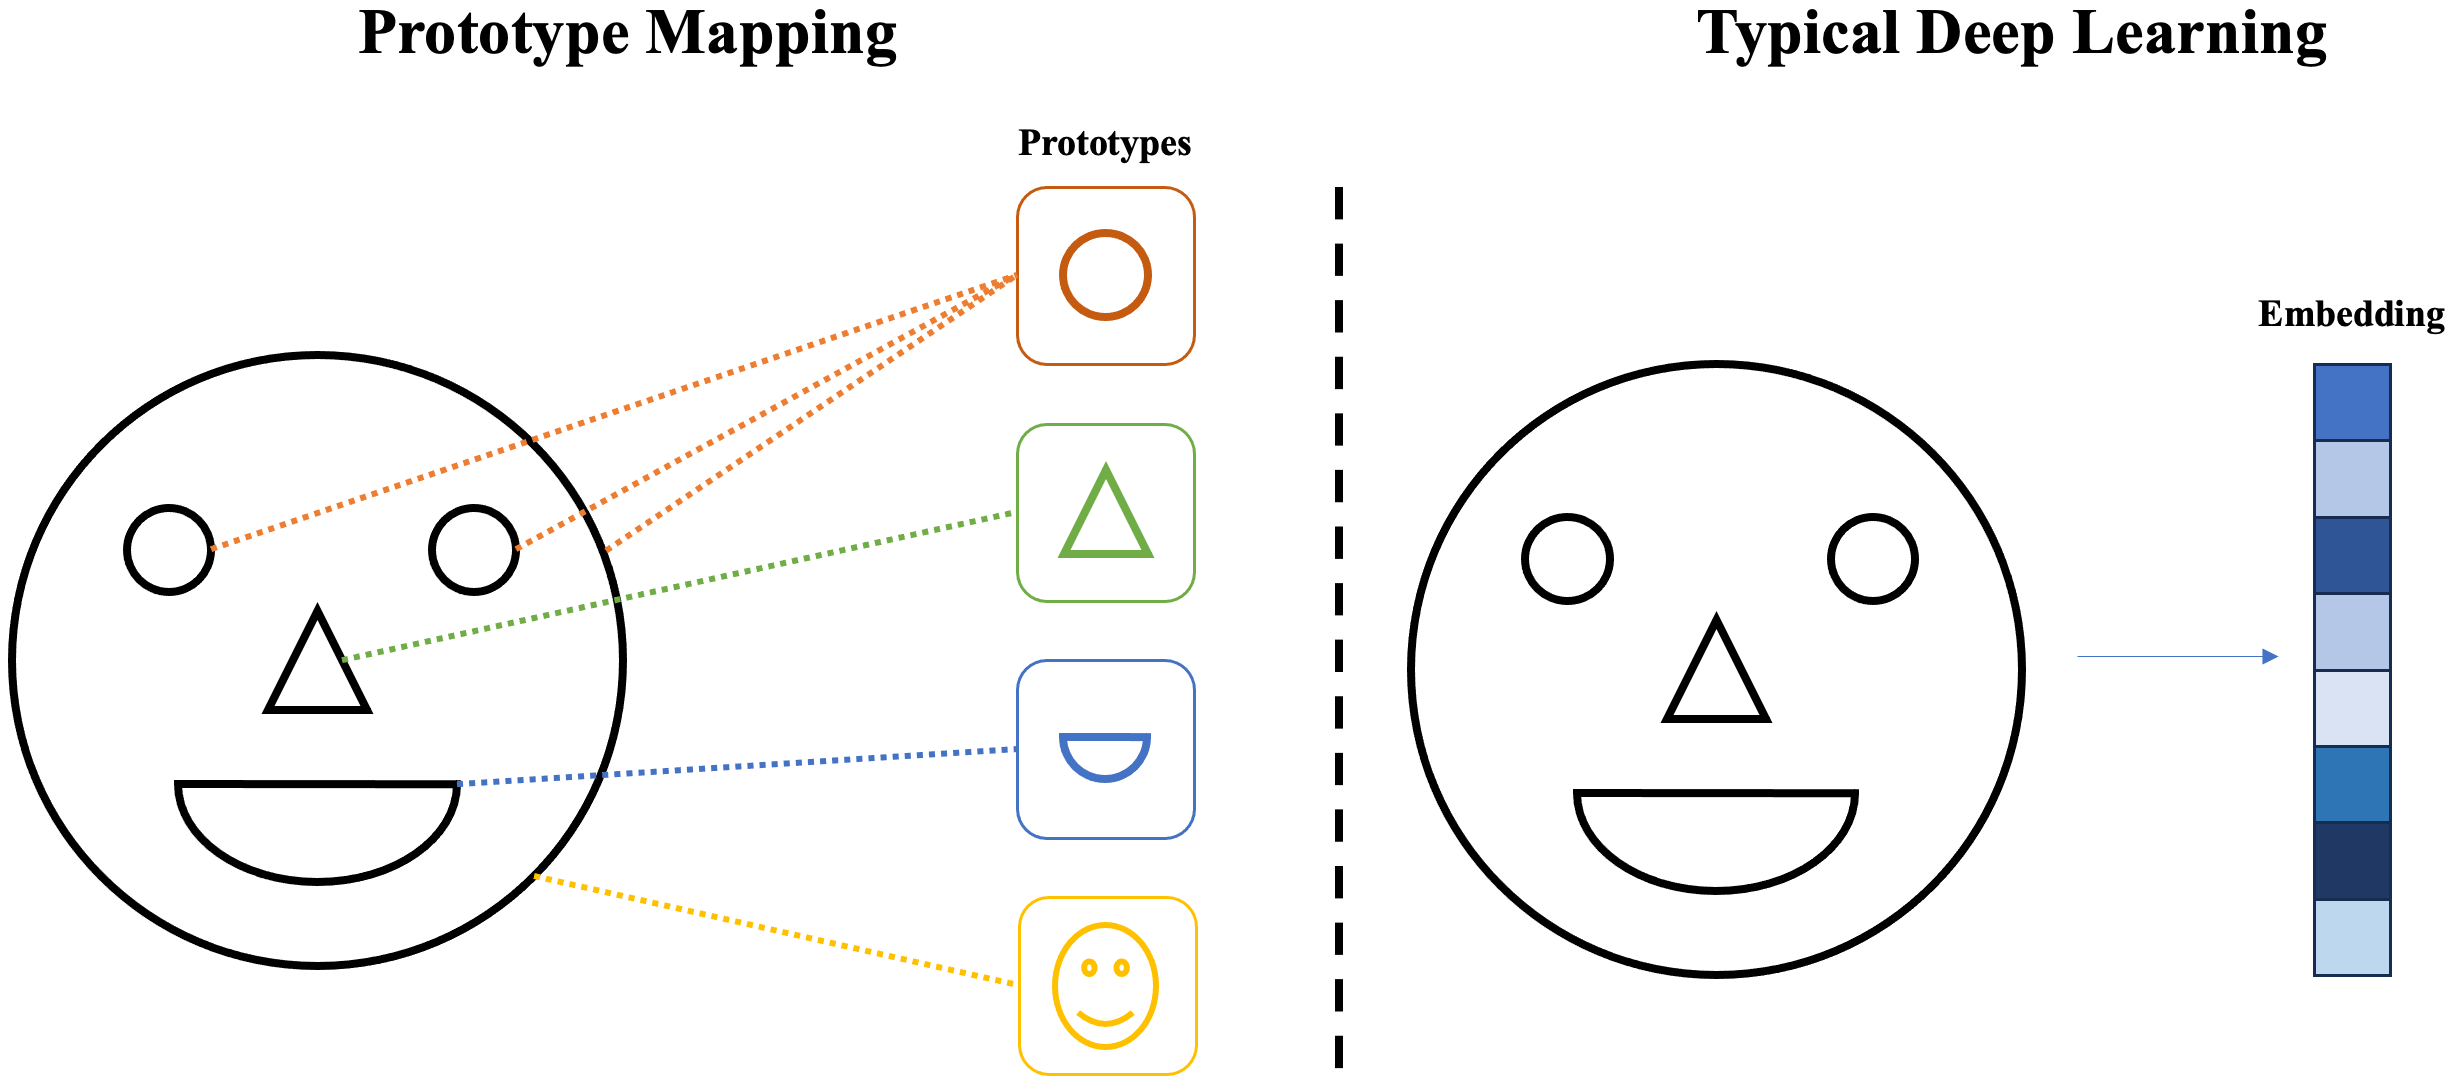
\includegraphics[width=0.99\textwidth]{prototype_mapping}
    \caption[Mapping from an image to prototypes]{Mapping from an image to prototypes and vice versa in contrast to deep learning models.}
    \figlbl{prototype_mapping}
\end{figure}

A system that avoids the fallacy of early commitment should fulfil the conundrum that local decisions are taken on the basis of plausibility in the light of high-level patterns, while high-level patterns can only be defined on the basis of low-level features.
The only solution is to iterate between local and global features, refining them in a coarse to fine manner \sidecite{wiskott_face_1996, wolfrum_recurrent_2008}. This process requires a two-way mapping from local features to prototypes and vice versa, as visualized in \figref{prototype_mapping}.
Thus, the system should be able to map parts of an image to meaningful prototypes, as shown on the left, and not just compress the entire image to an embedding representation as typically done in deep learning applications \sidecite{prince_understanding_2023}.
Such systems have been explored in the theory of self-organising projection fibres (c.f. \secref{projection_fibres}), however, did not yet scale to natural images except for human faces \cite{wolfrum_recurrent_2008}.

This section describes a system that might scale to natural images.
It is based on three main components: A sensory stage \emph{L0} that extracts features from the image, a stage \emph{L1} building local features, and a stage \emph{L2} mapping these local features to object prototypes by utilising projection fibres.
In the context of biology, the sensory stage \emph{L0} could stand for the eyes translating visual information into neuronal activity, \emph{L1} could stand for the primary visual cortex \sidecite{tong_primary_2003, grill-spector_human_2004}, and \emph{L2} for an area in the temporal cortex \sidecite{miyashita_inferior_1993, conway_organization_2018}.
These three building blocks are described in the following.

\subsection{Building Blocks}
\begin{figure}[h]
    \centering
    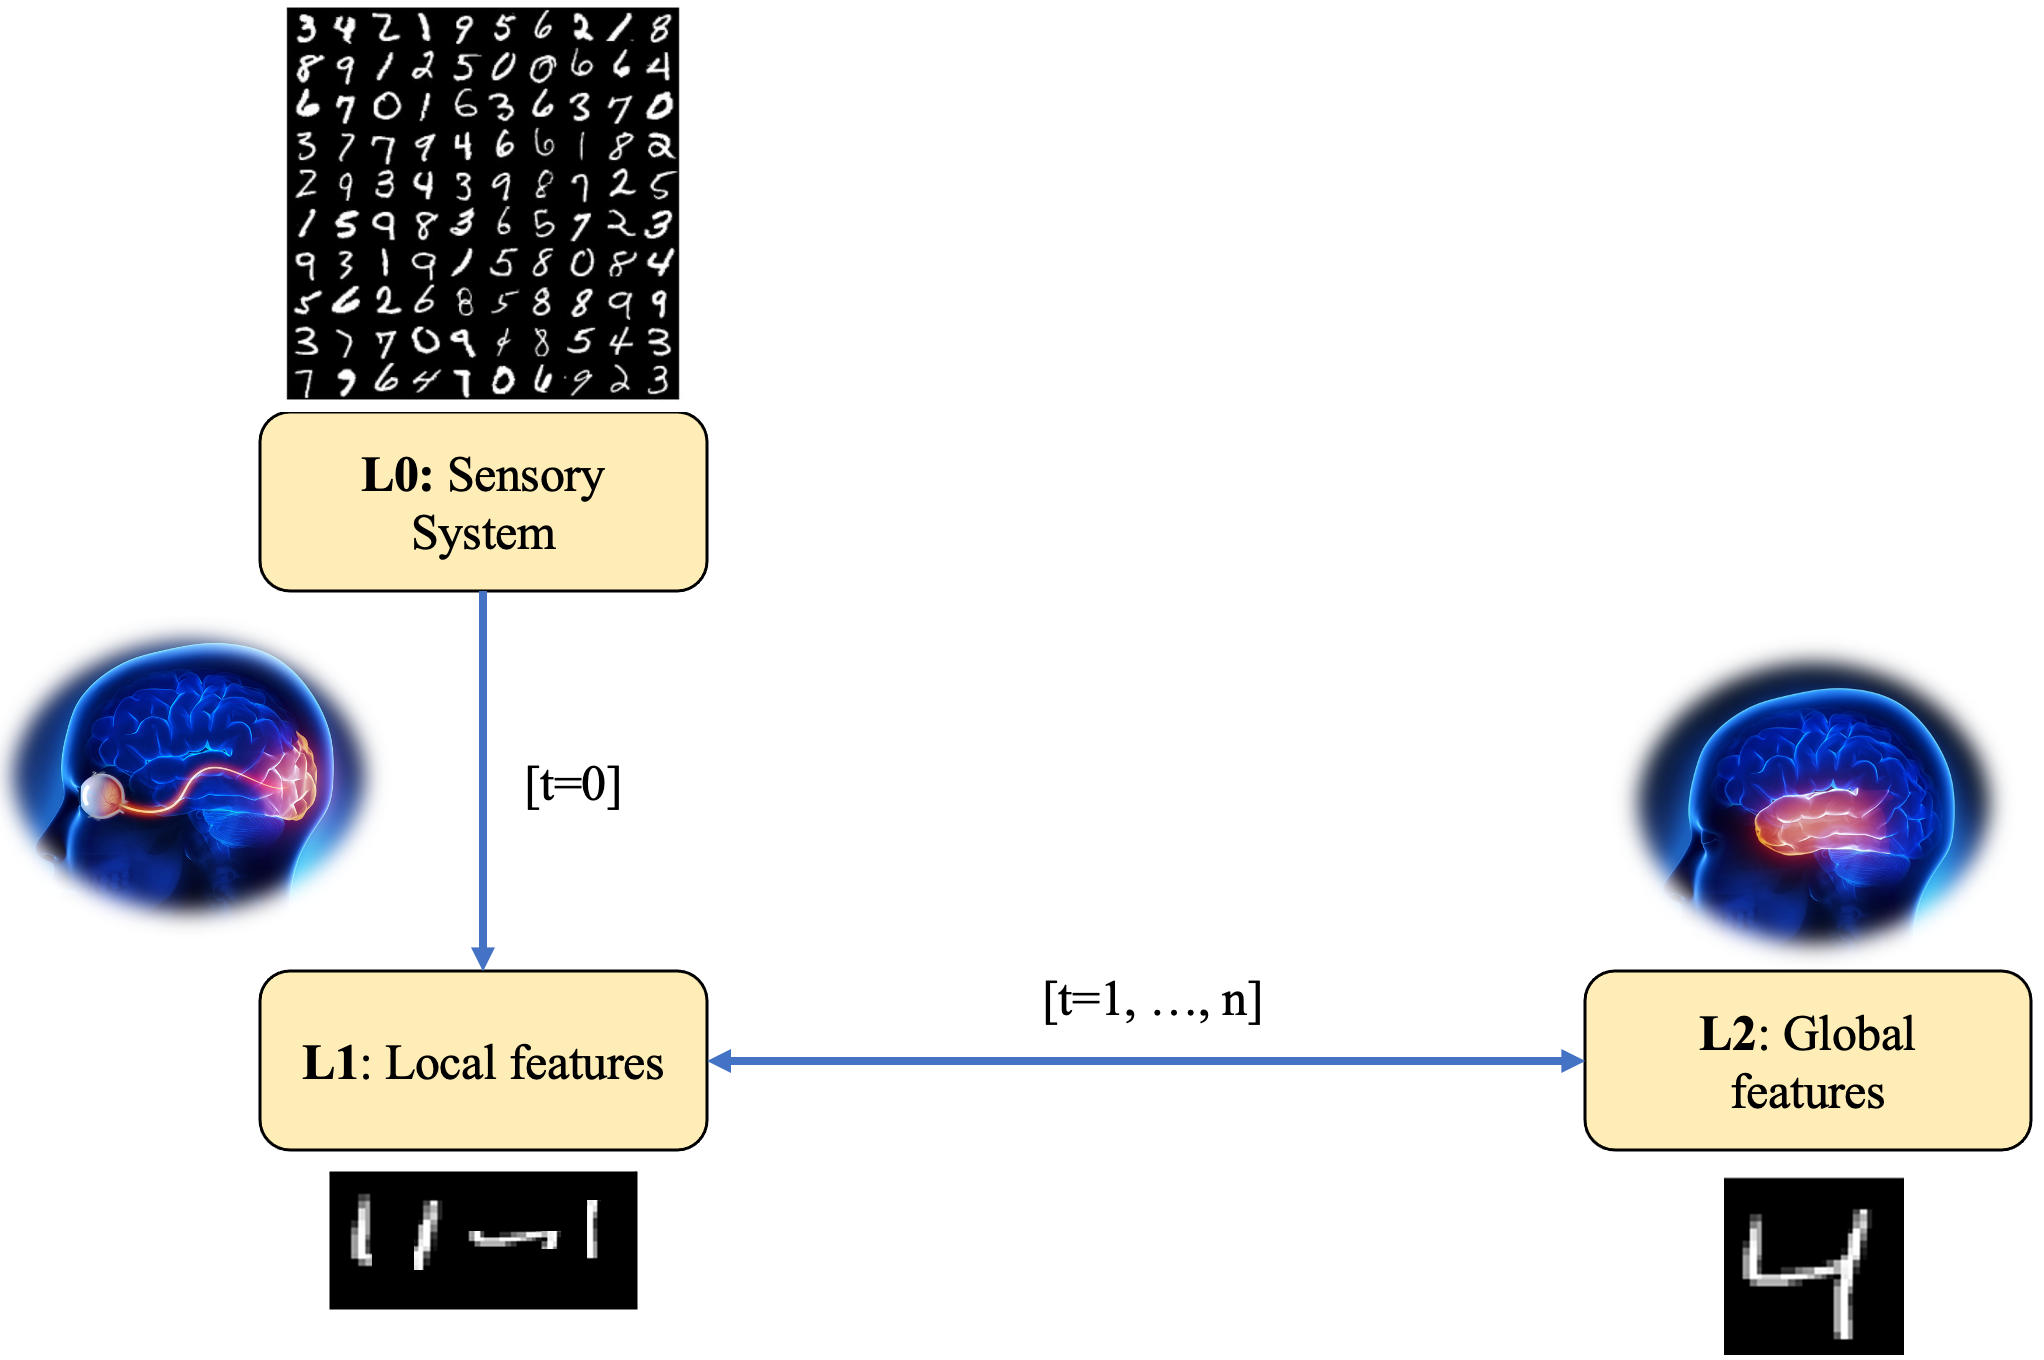
\includegraphics[width=0.99\textwidth]{system ovierview}
    \caption[Overview of the framework]{Overview of the framework. \emph{L0} extracts features from the image at timestep $t=0$, \emph{L1} builds local features, and \emph{L2} maps them to global features. The network refines the features over multiple timesteps by iterating between local and global features.}
    \figlbl{system_overview}
\end{figure}

\figref{system_overview} provides an overview of the building blocks of the proposed framework. The Sensors system \emph{L0} is only active once and extracts features. These features are refined over multiple timesteps by iterating between local and global feature processing, thereby preventing the system from early commitment.

\paragraph{Sensors System \emph{L0}.} The sensory stage \emph{L0} extracts features from the image that are forwarded to \emph{L1}.
A typical input to the sensory stage is an image having one (grayscale) or three (RGB) colour channels. Therefore, such an image can be interpreted as having one or three features at every spatial location.
The sensory system extracts multiple higher-level features by considering a spatially local neighbourhood. Thus, the number of features is increased by the sensory system.
A sensory system can be, for example, the first layer of a pre-trained CNN model.

\paragraph{Local Features Stage \emph{L1}.} The local feature stage is a single layer with short-ranging lateral connections \sidecite{gilbert_lateral_1990}, allowing neurons in a spatially narrow neighbourhood to support each other. Lateral connections can be considered recurrent connections operating at the same level of features. Input from the sensory system activates some feature neurons in \emph{L1}. However, their continued firing relies on receiving support from a sufficient number of other activated neurons that are laterally connected to them. Initially activated neurons that do not receive enough lateral support deactivate after a short period due to inhibition \sidecite{coombs_specific_1955}.

The lateral connections are learned through self-organisation. Patterns occurring repeatedly in the training data will constantly activate the same cells simultaneously. Using Hebbian learning strengthens the connection between these cells, and the pattern is ``stored'' in a net fragment. The inhibition strength increases during training so that only frequently occurring patterns can lead to constant cell activation.

Consequently, many neurons might be activated by the sensory stage, but only the ones supporting each other remain active.
Therefore, it is essential to view the process from the perspective that the winning neurons are integral parts of consistent net fragments, enabling them to persist.
The connections present in \emph{L1} possess the capacity to represent an extensive array of consistent connectivity patterns. Each neuron within \emph{L1} exhibits multiple excitatory incoming and outgoing connections, allowing it to be involved in slight variations and deformations of a specific pattern and completely distinct global patterns. However, due to the limited range of lateral connections, coherence is maintained only within that particular range.

\paragraph{Global Features Stage \emph{L2}.} Long-range connections are essential to represent larger-scale structures like an object. In \emph{L2}, large patterns, typically representing objects, are stored. 
It has a smaller coverage area, focusing specifically on object-centred representations rather than encompassing the entire visual field.
The patterns in \emph{L2} remain invariant to translation, scale, and orientation, enabling the incorporation of broader spatial relationships.

In the object recognition process, corresponding net fragments in \emph{L1} are mapped to object prototypes in \emph{L2} through active projection fibres. Here, ``corresponding'' refers to neurons relating to the same point on the object's surface.
The projection fibres between \emph{L1} and \emph{L2} are composed of ``maplets''. A maplet comprises a collection of fibres that establish one-to-one connections between all neurons in a small patch of \emph{L1} and all neurons in a small patch of \emph{L2} in a topological manner. This topological connection links neighbouring neurons in \emph{L1} to neighbouring neurons in \emph{L2}. Both \emph{L1} and \emph{L2} are divided into overlapping patches, and for each pair of patches — one in \emph{L1} and one in \emph{L2} — a corresponding maplet exists.

Control units are used to activate projection fibres.
Control units initiate activation when they observe a high pattern correlation between the fibres reaching \emph{L1} and \emph{L2}. They inhibit competing units and stabilize the network in \emph{L2} using the activated fibres. Consequently, the activated projection achieves a homeomorphism, where neurons of a particular feature type in \emph{L1} are connected to neurons of the same type in \emph{L2}.


\paragraph{Bernoulli Neuron.} The limited interpretability of deep networks is one of the reasons why they cannot always fully leverage their potential and be used, for example, in safety-critical applications \sidecite{gerasimou_importance-driven_2020, li_interpretable_2022}.
This is especially due to the fact that the activation of artificial neurons can be any floating point number, giving a neuron the capability to represent an infinite number of states. This limits interpretability as it is unclear what these neuronal activity strengths actually mean.
Furthermore, it hinders networks from forming proper net fragments: An input image depicting a pattern creates activation within the network, and the cells that respond to that pattern should strengthen their connections. However, unique patterns should activate a unique group of cells. With floating point numbers as cell states, different patterns can activate the same cells with different magnitudes and might hinder forming proper net fragments.
Therefore, all proposed building blocks are based on neurons that sample their activity from a Bernoulli distribution and thus are binary (c.f. \secref{bernoulli_neuron}).
Such neurons are highly interpretable, as they are either turned on or off, depending on the pattern presented at the network's input.
Furthermore, binary neurons increase robustness to noise \sidecite{Ahmad_Hawkins_2015}.


\subsection{Relation to Theory of Natural Intelligence}
The mapping between input data and stored object prototypes is closely related to the human brain's functionality and in line with findings from neuroscience \cite{kandel_principles_2013, olshausen_emergence_1996, vogels_inhibitory_2011, payeur_burst-dependent_2021} and psychology \cite{ellis_source_1938, kohler_gestalt_1992, wagemans_century_2012, hamlyn_psychology_2017}.

The theory of natural intelligence by \sideciteay{von_der_Malsburg_Stadelmann_Grewe_2022} describes how the brain develops an overlay of net fragments (c.f. \secref{natural_intelligence}). These attractor networks consist of neurons supporting each other to remain active.
This behaviour is implemented in the local feature stage \emph{L1}: The sensory signal from \emph{L1} activates many neurons from which only the ones receiving enough lateral support remain active. The neurons that support each other thus build a net fragment.

The theory also describes that an object is represented by multiple net fragments, whereby each net fragment represents a part of the surface of that object.
As described above, net fragments are built in \emph{L1} but are restricted to a spatially local neighbourhood. Projection fibres map these net fragments to object prototypes in \emph{L2}. Thus, an overlay of attractor networks represents an object, as suggested in the theory of natural intelligence.

Furthermore, it is postulated in the theory that self-organisation is the key algorithm to form such fragments and the learning mechanism loops between activity and connectivity for a short time until an attractor state is reached.
In the context of this work, self-organisation is used to organise the lateral connection in \emph{L1}. In fact, local Hebbian learning is applied to learn the support strength between neurons, allowing the network to turn off neurons that are not part of the dominating net fragments.
Furthermore, looping between activity and connectivity is implemented with projection fibres. 
Each prototype in \emph{L2} is considered a hypothesis of what object is present in the input. A net fragment can be mapped to multiple prototypes, and each active net fragment supports specific hypotheses in \emph{L2}. The hypotheses act back on \emph{L1} and, in turn, support local net fragments. Thus, the activity part is realised by \emph{L1} when supporting or turning off cells and the connectivity part is realised by projection fibres mapping the net fragments to \emph{L2}, thereby providing feedback to \emph{L1}.

Overall, I argue that the proposed framework is an implementation following strictly the theory of natural intelligence \cite{von_der_malsburg_theory_2022}. Thus, according to leading experts in the field, this framework has the ability to make a step towards natural intelligence. However, not all parts have been incorporated yet. For example, the framework is still limited to processing images and cannot yet deal with multi-modality. However, incorporating multi-modality can be done similarly to the principle of the vision processing system (c.f. \secref{framework_multi_modality}).


\subsection{Advantages}\seclbl{framework_advantages}
The proposed framework is expected to have various advantages over the typical deep learning setting. These are described in the following.

\paragraph{Ambiguity.} The proposed framework permits the persistence of multiple net fragments, enabling the system to handle ambiguity effectively. For example, when presented with a face comprised of distinct objects (c.f. \figref{sdp_mountain}), both the subnetwork responsible for abstract faces and the subnetworks associated with individual objects become active concurrently. Consequently, one can attend to these subnetworks simultaneously, utilizing attention in its original sense rather than the conventional deep neural network (DNN) interpretation \sidecite{niu_review_2021}. I speculate that this represents a fundamental distinction from neural networks that are compelled to represent the entire scene within a single high-dimensional dense vector.

\paragraph{Interpretability.} The framework allows for much better interpretability than classical deep networks. Each neuron is binary and can be part of a multitude of subnetworks and thus has a semantic meaning, i.e. corresponds to something meaningful. Furthermore, every neuron's internal state is a probability that can be interpreted as the network's confidence that this specific feature was observed in the input. A network of probabilistic neurons that support each other over timesteps can also be interpreted as a directed graph. This allows to trace how subnetworks are activated. 
Furthermore, the projection fibres map net fragments to object prototypes, making it much simpler to understand the network's decision process for object detection.
Without formal proof or presenting an interpretability framework, I speculate that using this framework will significantly simplify the explainability of intelligent systems.

\paragraph{Robustness.} A neural network is usually represented with a vector which is sequentially processed by mathematical functions (e.g. with neural layers). Artificial networks, in particular, are not robust to noise and are susceptible to adversarial attacks \sidecite{Akhtar_Mian_2018}. Slight changes to the input or a network-internal vector can completely falsify the overall result. This is because typical artificial networks work with continuous numbers, and these feature vectors can consequently lie anywhere in the feature space. Therefore, a minimal change, e.g. triggered by noise, can shift the feature to the other side of the decision boundary and change the result. A binary vector, on the other hand, has different mathematical properties and is more robust against noise and adversarial attacks, especially if they are sparse and distributed\sidenote{Only a small portion of the bits are ``on'', and representations differ by multiple binary bits.} \sidecite{Ahmad_Hawkins_2015}.
Subsampled or noisy vectors are still semantically similar and are close to the original vectors when compared, for example, by counting the overlap of bits between two vectors.

\paragraph{Processing Duration.} A neural network usually processes input for a fixed number of iterations. The proposed framework has an adaptable processing duration: The activated prototypes in \emph{L2} can be interpreted as hypotheses, which are refined until a consensus, i.e. an attractor state, is reached. This happens rather fast if the local features can be unambiguously mapped to one of the prototypes and requires more iteration between \emph{L1} and \emph{L2} if it is unclear to which prototype the local features belong to or if the input is ambiguous. Thus, the processing duration can be automatically adjusted to the input data.

\paragraph{Object-Independent Transformations.} The same projection fibres are applied to all object prototypes, allowing to learn object-independent transformations. For example, an object might be slightly stretched, rotated, or deformed compared to the stored prototypes. The projection fibres learn to ignore such slight deformations independent of the object type. This allows the architecture to learn transformation invariance and to transfer this capability to new objects that have not been transformed in the training data.

\subsection{Multi-Modality}\seclbl{framework_multi_modality}
This work focuses on a framework for computer vision. However, the architecture has broader applicability and can be used for processing different sensor signals and be used in multimodal settings \cite{ngiam_multimodal_2011, liu_learn_2018, baltrusaitis_multimodal_2019}.
Having similar cell architectures processing different kind of signals is also in line with findings from neuroscience \sidecite{mountcastle_organizing_1978, mountcastle_columnar_1997}.

In the case of images, net fragments in \emph{L1} represent learned visual patterns that are part of an object's surface and are mapped with protection fibres to object prototypes that describe the visual appearance of objects. 
The same architectural structure can be applied to other types of signals. For example, an alternative sensory system could perceive audio signals. In this scenario, the local support in \emph{L1} would extend over nearby frequency ranges and time intervals. Consequently, phonemes or syllables could be learned locally and represented by net fragments. In the second stage (\emph{L2}), a sequence of phonemes or syllables could be mapped onto word prototypes.

Different sensory systems could even have separate domain-specific \emph{L1} layers in a multimodal setting, while the prototypes in \emph{L2} could be shared across modalities. This arrangement would allow to integrate different sensor signals and facilitates the creation of internal object representations with multiple modalities.


\section{Bernoulli-Sampling Neuron}\seclbl{bernoulli_neuron}
In traditional neural networks, neurons exhibit dense activity, meaning that even with applying the rectified linear unit (ReLU) activation function (c.f. \eqref{act_functions}), many neurons remain active (above zero) \sidecite{rhu_compressing_2018}, even though it is known that sparsity can improve results \sidecite{ide_improvement_2017}. Consequently, most synapses are active, and a neuron is represented as the weighted sum of many neurons from the previous layer without incorporating lateral connections. Furthermore, temporal dynamics are absent, as neural networks are typically perceived as functions that promptly process an input and generate an output. However, biological neurons have different characteristics than artificial neural networks \sidecite{kandel_principles_2013}:

\begin{itemize}
    \item A neuron is active when a relatively small amount of synapses are active (10 out of 10'000 connections). 
    \item Activation is sparse, i.e. at each point in time, only a fraction of neurons are active.
    \item Neurons that tend to fire simultaneously tend to form stronger bonds (Hebbian update rule).
    \item The connections are also lateral and not feed-forward only. This implies a time dependency used to form the net fragments. 
\end{itemize}


This suggests that implementing net fragments, similar to the human brain, requires using different principles than the ones used in classical neural networks. Therefore, a probabilistic neuron that samples its activation from a distribution is introduced.
Such a neuron is a binary neuron that does not fire when a certain threshold is reached but uses its internal state as firing probability.

A probabilistic neuron $x_i$ in the context of net fragments is modelled as a probability density function of the form:
\begin{equation}
    p(x_i = \text{active} | \text{activity of neighborhood}, \text{environment}) 
\end{equation}

Thus, the probability of a neuron being active depends on the activity pattern of the neurons in its local neighbourhood and factors of the environment (e.g., inhibition or presence of neurotransmitters).
Such a neuron can be implemented using a Bernoulli distribution, i.e., $B(p) = P(X = 1) = p = 1 - P(X=0)$. Having a neuron whose firing probability $p$ is governed by the neighbourhood activity and the environment allows to implement the behaviour of net fragments: After receiving an input, the neurons get excited and fire with a higher probability. However, their fire probability decreases quickly if not supported by neighbouring neurons. Thus, uncertainty and potential net fragments govern timestep 0 while shortly after the network reaches an attractor state. 

\subsection{Properties}
TODO: This section sounds bad

The proposed neuron implements a stochastic process and thus can flip, i.e. can fire even when the firing probability is low or vice versa.
This leads to noise in the network's activations.
However, this noise can be considered as normalisation mechanism within the network, similar to dropout layers \sidecite{TODO}.
Having neurons that might flip enforces the network to learn parallel paths and to ignore noise.
Similar to dropouts, the stochastic process can be deactivated during inference by using a fixed threshold of $0.5$. This leads to a more stable network during inference.
Having many binary neurons and sparse network activations increases robustness \cite{Ahmad_Hawkins_2015}.

Furthermore, binary neurons with an activation probability as internal cell state leads to much better interpretability as described in \secref{framework_advantages}.
Each neuron represents one single property as its state is binary, and the internal cell state describes how high the probability is of having that property observed.


\subsection{Practical Considerations}
TODO: This section sounds bad

A network layer processing images consists of $n_{\text{cells}} = C\cdot H \cdot W$ cells, $n_{\text{cells}}$ typically beeing a large number.
Thus, many neurons fire based on a probability distribution. In order that the network is not dominated by noise, it is important that the probabilities are not distributed around a mean $\mu = 0.5$.
Otherwise, most neurons have a high uncertainty if they should fire, leading to many neurons that fire randomly.
This is an issue especially at the beginning of training, when the network is dominated by uncertainty.

This issue can be migigated by pushing the activation probabilities towards $0$ or $1$. A simple solution is to use the Softmax function or to use the activations to the power of a factor $s$, i.e. $\boldsymbol{a} := \boldsymbol{a}^s$. The softmax function pushes the probabilities equally towards $0$ or $1$, while using a large factor $s$ pushes most activations towards $0$ while only the high probabilities remain high.
The advantage of using a factor $s$ is that it is adjustable, i.e. can be high at the beginning and constantly be decreased towards $1$ during training. Thus, it allows to scope with the uncertainty that dominates the network at the beginning and is reduced during training.
























\section{Model Overview}
%Overview 2-Staged Model (3 Components: Sensory System, L1, L2)
%For each stage: Motivation (what does the stages do)
%For each stage: Biological inspiration
%Processing loops: Multiple views per image, multiple steps per view
%Timesteps: Sensory system captures data at t=0, iterate between \emph{L1} and \emph{L2} for t=1, …, T


\subssection{Sensory System}
%Possible Implementations: Fixed filters (e.g. Gabor), learned filters (e.g. pre-trained CNN layers)


\section{L1}
% Subnetworks: Description and advantage
% Hebbian learning to build lateral support
% Distance of lateral connections
% Limiting lateral support with inhibition & normalization
% Alternative cells for alternative patterns
%%% Competition between graphs of lateral support structures
% Incorporating feedback from L2
% Implementation using convolutional operations
%%%  Initialization (self-support)
%%%  Measuring support goodness

\section{L2}
% Projection fibres and L2: Description and advantage
% Structuring of \emph{L2} -> unclear, might require some iterations to define?
% How to map \emph{L1} to L2-> unclear, might require some iterations to define?
% Providing feedback to L1-> unclear, might require some iterations to define?



\section{Implementation}
TODO Add Overview of entire system


\subsection{Processing Loops}
\begin{figure}[h]
    \centering
    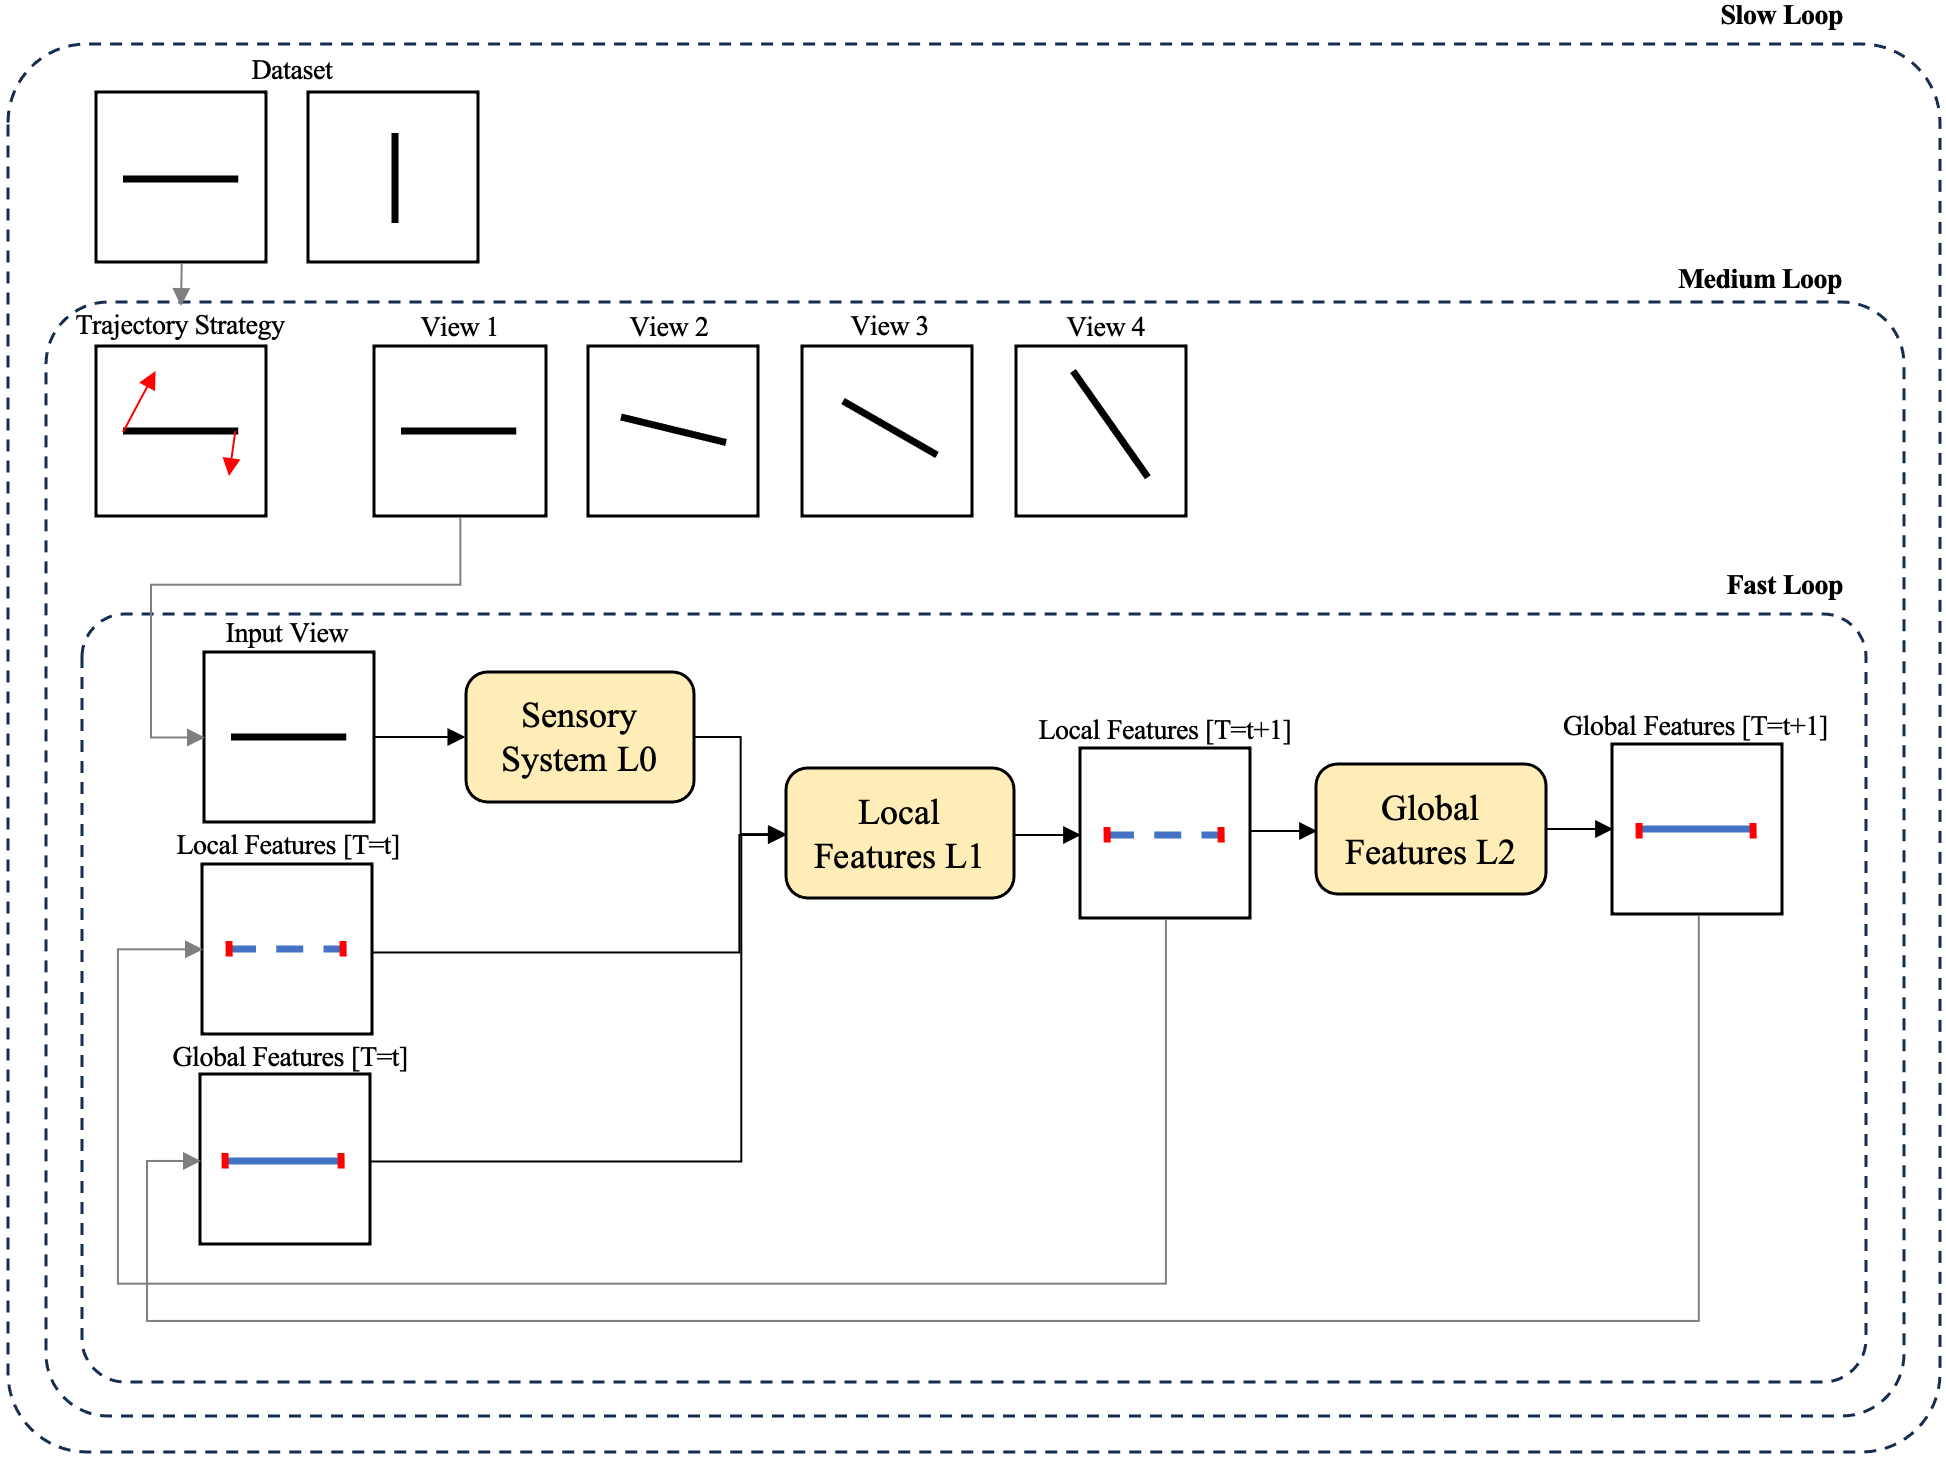
\includegraphics[width=0.99\textwidth]{lateral_loops.png}
    \caption[Processing loops of the network]{Processing loops of the network. From each sample in the dataset (slow loop), multiple views are generated (medium loop), and each view is processed over multiple timesteps by the model (fast loop).}
    \figlbl{lateral_loops}
\end{figure}
The proposed framework introduces nested learning cycles, each with a different functionality. Since the proposed framework runs on a tacked computer hardware, the cycles are bound to fixed timesteps. At each timestep, the innermost loops executes a step. As soon as the innermost loop is finished, an outer loops takes a step and the process is repeated.

\begin{itemize}
\item[\textbf{Slow Loop}] The dataset comprises $D$ images, with each image depicting a randomly generated line. The images are processed one after the other, building the outermost loop.
\item[\textbf{Medium Loop}] For each image in $D$, $V$ different views are sampled by slightly changing the image based on a trajectory strategy. This generates $V$ distinct yet visually similar images. Similar to our visual system, which captures multiple frames of an object before moving on to the next, this loop allows to perceive objects from various viewpoints.
\item[\textbf{Fast Loop}] From each view $V$, a sensory system creates neural activity that is processed by the network for $T$ timesteps. This loop allows the network to build subnetworks over several timesteps. First, the network has a high neural activity, which is quickly reduced within these $T$ steps as only the activations with enough lateral support remain active and convergence to an attractor state. At each timestep, the input (static) input from the sensory system as well as the previous cell state is fed into the network. The input of the sensory system is fed into the network to make it more stable. Intuitively, this can be compared to closing our eyes: When closing our eyes, we tend to forget the exact location of objects and thus our internal representation slightly shift away.
\end{itemize}


\subsection{Sensory Input}
An intelligent agent may have a multitude of sensory input. The main difficultly is that sensory input (especially images) are in continuous space, and they must be translated into an activation potential.
Thus, the sensory input must be linked to probabilistic neurons. Such a sensory system can be implemented by using either Gabor filters \sidecite{Gabor_1946, Granlund_1978} or, in a more advanced setting, with learned filters.
Such filters can be learned, for example, by training a deep network in a autoencoding setting \sidecite{rumelhart1985learning}. Even though such networks violate the principles from the Gestalt phenomena \cite{ellis_source_1938, kohler_gestalt_1992, wagemans_century_2012, hamlyn_psychology_2017}, their first layer exhibit excellent capabilities in extracting relevant features from images. Therefore, I argue that such filters are well suited as a network's sensory system if only the first layers are kept. However, also the output $\boldsymbol{h}$ of such as layer is not binary.
One option is to consider the normalized values of $\boldsymbol{h}$ as probabilities, with the notion that higher values indicate regions where a filter discovers matching features in the image. Alternatively, another approach involves setting all values in $\boldsymbol{h}$ above a pre-defined threshold to 1 and assigning 0 to the remaining values.
As a third option, quantization networks such as VQ-VAEs \sidecite{NIPS2017_7a98af17} can be used to map local features to a discrete value that can be translated in a binary activation pattern.

This thesis focuses on implementing a proof-of-concepts for handling straightforward images, which allows the utilization of a pre-defined hand-crafted sensory system. However, when processing complex natural images in future research, it is imperative to conduct empirical investigations to explore these possibilities further.

\subsection{Feature Extractor (L1)}
\begin{figure}[h]
    \centering
    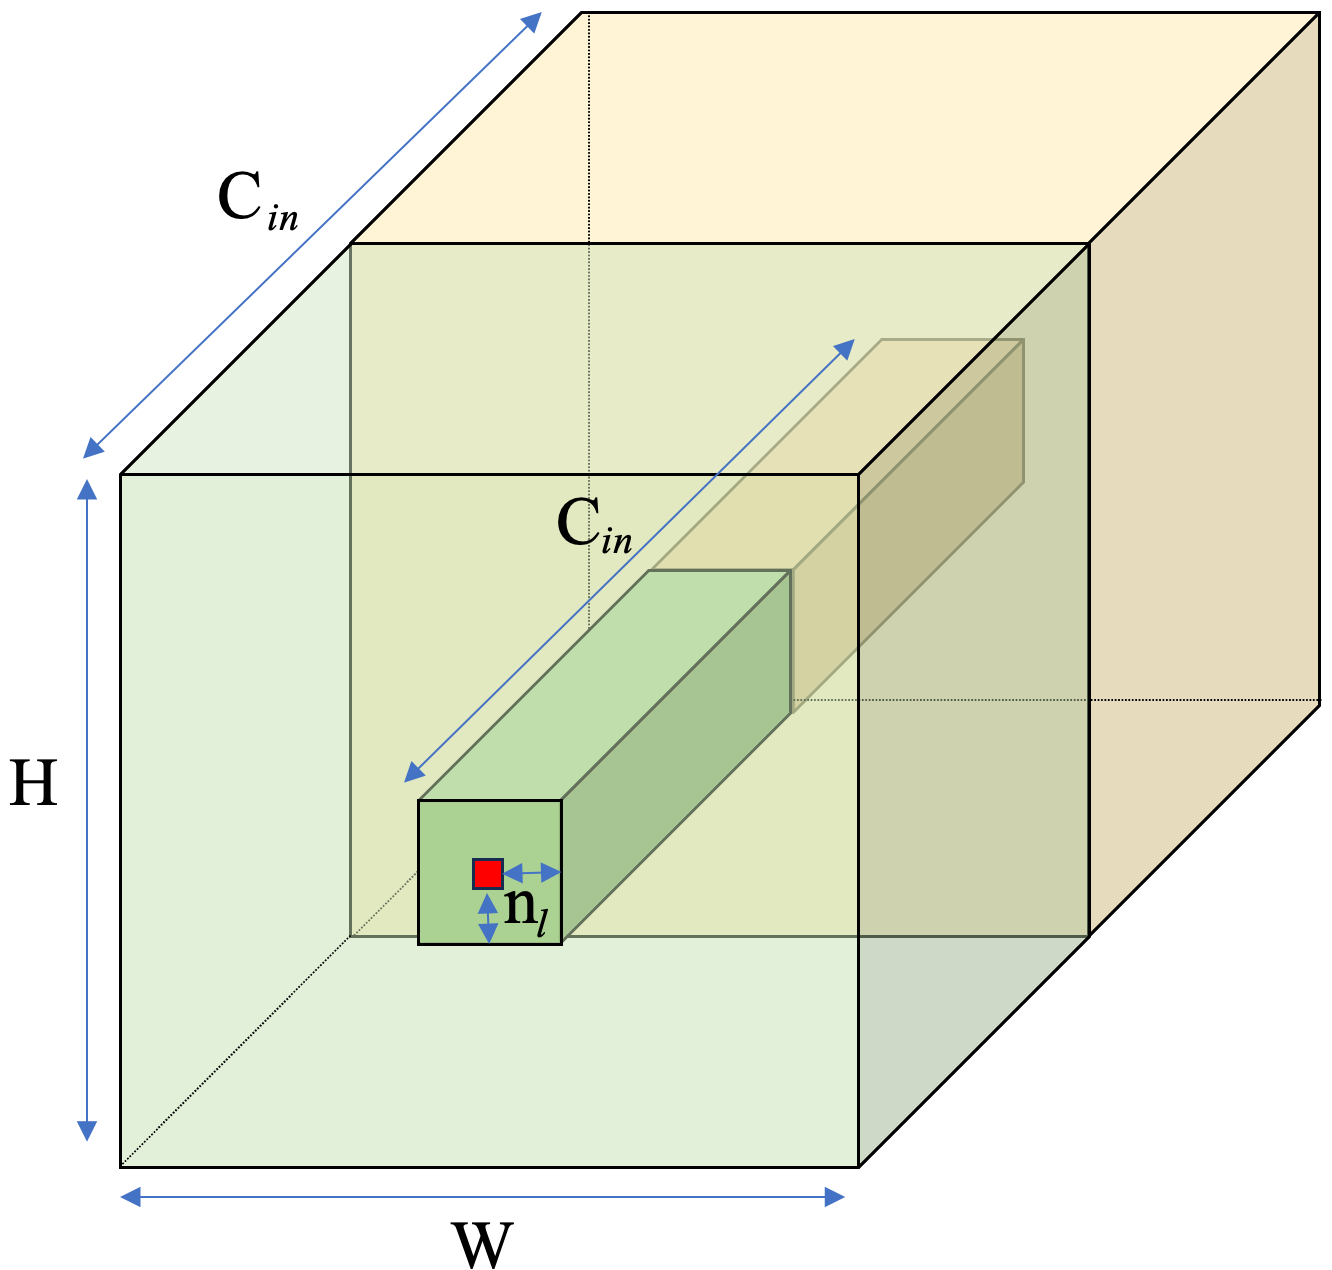
\includegraphics[width=0.99\textwidth]{local_neighbourhood.png}
    \caption[Laterally connected cells]{Visualization of the laterally connected cells: The red cell of an array of cells of the size $C \times W \times H$ is laterally connected to an neighbourhood of size  $C \times 2n \times 2n - 1$ ($-1$ representing the red cell itself).}
    \figlbl{local_neighbourhood}
\end{figure}
The sensory system converts an image into a binary observation of size $C_{in} \times W \times H$ where $C_{in}$ is the number of input channels, $W$ the image width and $H$ the image height.
Our network implements one cell for each binary observation, leading to $C_{in} \times W \times H$ cells.
Having multiple input channels means having multiple cells at the same pixel location, representing one of $C_{in}$ feature.

Let's denote a cell of feature channel $c \in \{0, ..., C_{in}\}$ at position $w \in \{0, ..., W\}$, $h \in \{0, ..., H\}$ as $x_{c,w,h}$.
Each cell's activation is supported by neighbouring cells through lateral connections. Let's define the reach of lateral connections along the vertical and horizontal axis of an image as $n$.
Furthermore, the cells are also laterally connected across the channels, allowing a cell be supported from other cells representing different features.
Therefore, each cell has $C\cdot n^2 - 1$ laterally connected cells at the positions $\{x_{0,w-n,h-n}, ..., x_{C,w+n,h+n}\} \\ x_{c,w,h}$. This lateral connectivity is also depicted in \figref{local_neighbourhood}. 

A known pattern should excite the cells and the cells should remain active through lateral support. 
However, the pattern can appear at any position within the image, requiring the lateral support to be position equivariant.
Computer vision architectures solve this problem with convolutional filters shifting over each pixel location. This mechanism can also be used for implementing the lateral connections: When using a convolutional kernel with size $C_{in} \times 2n+1 \times 2n+1$, the state of a cell is updated based on the local neighbourhood. This local neighbourhood are the laterally connected cells and the learned weights of the kernel is the weight of their support.
Thus, lateral support is implemented as


\begin{align}\eqlbl{convlat_1}
	\Delta w_{ij} = \eta x_i x_j
\end{align}


\subsubsection{Hebbian Updates}
The human brain's learning algorithm is based on local self-orgnisation and unsupervised (or self-supervised) learning \sideciteay{von_der_Malsburg_Stadelmann_Grewe_2022}. The biologically most plausible learning algorithm is Hebbian learning \sidecite{Hebb_1949}. Hebbian learning can be summarized as ``neurons that fire together wire together'' (c.f. \secref{Hebbian}).
This learning rule is well suited for learning lateral connections: If two cells are active together (``fire together''), their weight is increased (``wire together''). During training, the cells are activated is a specific pattern based on the sensory input. Hebbian learning strengthens the connections between the cells that are active at the same time, i.e. increasing the lateral support between these cells. Furthermore, the weight (i.e. the strength of the lateral support) is reduced between between cells that fire in disparity (one of the cells is firing while the other is not).
Thus, Hebbian learning is the algorithm to learn lateral support while being biologically plausible.

The weight $w_{ij}$ between two binary cells $x_i$ and $x_j$ is increased, when they are active at the same time. The weight update $\Delta$ can be calculated as follows, leading to an increase of $w_{ij}$ by $\eta$.

\begin{align}\eqlbl{hebbu_1}
	\Delta w_{ij} = \eta x_i x_j
\end{align}

The formula above leads to an increase when both neurons are active at the same time. To decrease lateral support between cells where only one cell is active, the formula can be extended as follows:

\begin{align}\eqlbl{hebbu_2}
	\Delta w_{ij} = \eta \left( x_i x_j + (x_i-1) x_j + x_i (x_j -1) \right)
\end{align}

The term $(x_i-1) x_j$ becomes $-1$ if the $x_i=0$ and $x_j=1$ and thus decreases the weight if these cells are firing disparity. The second term $x_i (x_j -1)$ implements the same behaviour for the other cell ($x_i=1$ and $x_j=0$).

So far, only the update between two cells is discussed. However, the network consists of multiple cells whose lateral connection strength is defined by a kernel $\boldsymbol{W}$. This kernel has the size $C_{out} \times C_{in} \times 2n+1 \times 2n+1$. Thus, the activity of a cell is calculated based on different weights connecting all neighbouring cells.

During training, the network might see similar patterns multiple times, leading to very strong connections between specific cells. In order that these lateral connection strengths cannot grow to infinite, the weight is normalized. The weights are normalized per output channel, ensuring that the post-synaptic activity cannot get too high. 

\begin{align}\eqlbl{hebbu_2}
	\boldsymbol{W(C_{out})} = \boldsymbol{W(C_{out})} / (1\cdot 10^{-10} + \sqrt{\sum_{ci}^{C_{in}}\sum_{w}^{2n+1}\sum_{h}^{2n+1} \boldsymbol{W(C_{out},ci,w,h)}})
\end{align}


\paragraph{Breaking the Symmetry.}  Oja \cite{Oja_1982} showed that the Hebbian learning rule converges for linear neurons to the first principle component of the input data. He concluded that a 
network of such neurons appears not very useful, as all neurons will just learn the first principle component and that an additional element is required providing differentiation between the neurons.
In practice, this additional element is typically some kind of competition such as winner-take-all. With winner-take-all, only the neuron with the highest activation is selected for learning. In the case of of our network with lateral connections, this means that at each pixel location exactly one of the feature channels $C$ is updated. However, this not desirable: Imagine a pixel region with no activation: In this area, we don't want to learn any support between neurons as there is no activity. However, with winner-take-all, we enforce one channel to be active and thus learn lateral support between this enforced activity. However, we found that no measures are necessary at all. The probabilistic neuron is able to break the symmetry. When using the probabilistic neuron, neurons are activated with e certain probability. This probability provides enough differentiation between cells, 
making a competition strategy superfluous.

\paragraph{Implementation Details.} Implementing Hebbian updates efficiently in a deep learning framework is not trivial: In an efficient implementation, the kernel is not shifted from cell to cell but a circulant matrix is built so that all kernel updates can be calculated in parallel. However, by applying this operation, information about the cell's lateral influence is lost. One way to efficiently implement Hebbian learning for convolutional operations is to use special loss functions. Miconi \cite{Miconi_2021} proposes to use a loss function whose derivative is exactly the Hebbian update. By doing so, backpropagation of error can be used to update the weights. In this thesis, a different implementation is used that comes with a slight memory overhead but is very efficient and does not rely on backpropagation at all. Furthermore, it gives much more flexibility and allows to implemented different normalization strategies. Instead of using a forward pass through a convolutional layer with subsequent backward pass, my implementation uses two convolutional layers without backward pass. The first layer is a fixed, binary convolution that restructures each input patch into a single column vector. This is followed by a $1\times1$ convolution containing the actual weights. Specifically, we can pass the input through a fixed convolution with an input size of $C_{in} \times 2n+1 \times 2n+1$ and $C_{in} 2(2n+1)$ output channels. The weight vector for this convolution is set to $1$ for the connections linking input $c_i,w,h$ to output $c_iwh$ (where $c_i$ $w$, and $h$ range from 1 to $C_{in}$, $2n+1$, and $2n+1$, respectively), and it is set to 0 everywhere else. This process reorganizes the values of each input patch from the original convolution into non-overlapping column vectors, effectively duplicating them. Next, we can apply the actual weights of the original convolution using a simple $1\times1$ convolution. This can be achieved by performing a tensor product with appropriate broadcasting.


\subsubsection{Initialization}\seclbl{lateral_init}
\begin{figure}[h]
    \centering
    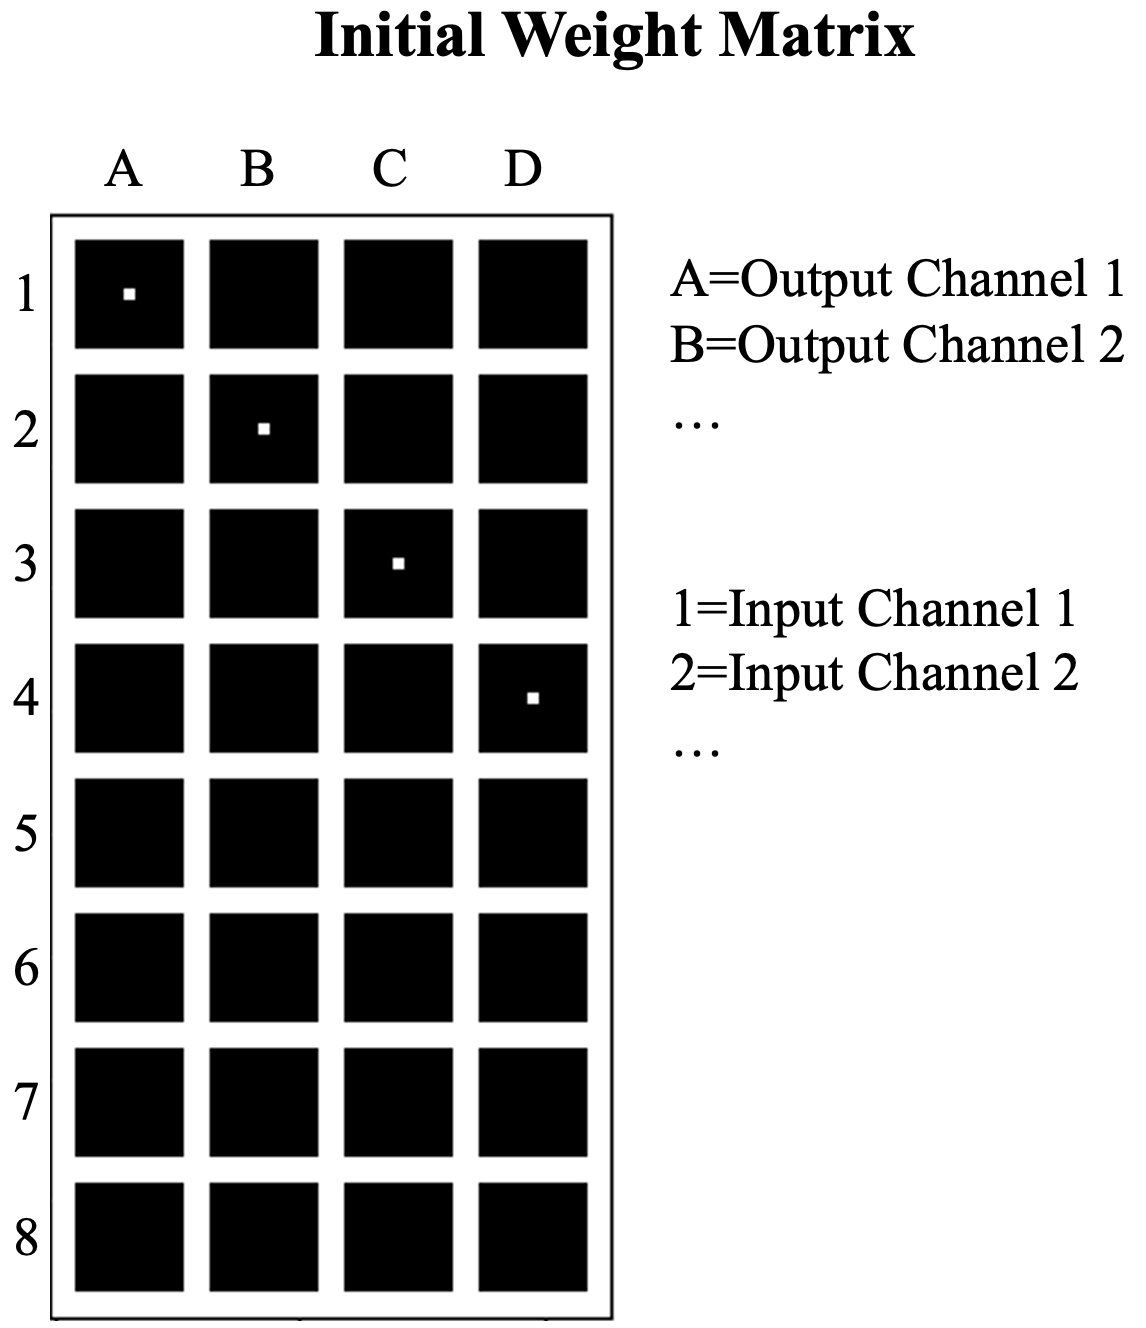
\includegraphics[width=0.99\textwidth]{lateral_init_weights.png}
    \caption[Initialization of the lateral weight matrix]{Initialization of the lateral weight matrix. The weight at the middle of a kernel, whose input and output channel have the same index, is set to $1$.}
    \figlbl{lateral_init_weights}
\end{figure}
The lateral support is implemented as weights of a convolutional kernels.
It is crucial to initialize these kernels properly, otherwise, the activations are not stable and typically converge to weights that either activate all cells or none cells.
For example, when the kernels are initialized with zeros, there is no lateral support and all cells will turn off immediately.
If the weights are initialized randomly, the initial support is random and patterns that are not in the training set  are supported.

I found that it works best if the weights are initialized with a high self-support, meaning each cell supports itself to remain active.
Self-support can be implemented by setting all weights of a kernel of size $C_{out} \times C_{in} \times w \times h$ to $1$ at the indexes that fulfil 
$C_{out} = C_{in}$, $w = n+1$, and $h = n+1$. Thus, the weight at the middle of a kernel that has the same input as output channel is set to $1$ while the other weights are set to $0$. This initialization strategy also works for kernels with a different number of input and output channels as shown in \figref{lateral_init_weights}.

Having such a weight matrix ensures that the cells activation at time $t$ and at time $t+1$ is exactly identical. However, after applying the Hebbian learning rule, the weights are updated in a way to capture the data's statistics.


\subsubsection{Normalization}
The lateral support defines the probability of a neuron to be active. However, the output of a convolutional operation is not in the range $0, ..., 1$ but can be any floating point number. Thus, this numbers have to be normalized to represent a probability.
Normalizing is quite challenging for the following reasons:
\begin{itemize}
	\item The lateral support increases over time: The lateral weights are initialized by only having self-support. However, the network's cells learn to support each other based on the data's statistics. This has the effect, that neurons become stronger activations during the course of the training process. For example, a single cell can have a binary value of $1$ at the beginning. This cell supports itself, i.e. keeps the $1$ at the beginning. After Hebbian updates, this self-support can either go towards $0$ and the cells turn off or can be supported by up to $n^2$ cells. The support strength of each of these cells can be in the range $-1, ..., 1$. Thus, a cell can have an activation up to $n^2+1$. The challenge hereby is that its initial support is $1$ and then evolves to a complete different value even if the data remains identical. Thus, the support needed to remain active must be low at the beginning of the training and be slowly increased during training until an upper bound is reached.
	\item The possible support depends on the input data: The sensory system extracts different features from the input data. Depending on the input data, there can be regions with a lot of detected features and regions with less features. For example, some areas can be constituted from many edges, and well pronounced structures leading to a lot of activations in various channels (e.g. a zebra within an image) while other areas have rather low frequencies and only a few activations (e.g. the sky in the background of the zebra image). However, even though areas have only a few activations, they should not just be turned off. Otherwise, the network would only keep features of areas with a high frequency and discard all other information.
\end{itemize}

Thus, the support depends on the learned lateral weights that change slowly during training and the input data that change every time a new scene is observed.
The problem with the changing weights can be solved by dividing the cells' activation by the sum of the lateral weights.
This normalization is done per feature channel. This allows to deal with the problem that different features receive a different strong support.
By doing so, more lateral support is needed to remain active when more lateral connections are learned: At the beginning, only self-support exists and thus the sum of the weight is $1$. Therefore, a cells activation is divided by $1$ and being active at time $t$ is enough to be active at time $t+1$.
However, during training, more lateral connections are build (i.e. more weights become $>1$). Therefore, a cells activation is divided by a value $>1$ and the activation has to be stronger to remain active with a high probability.
Mathematically, the normalization of an array of cells with an activation strength $\boldsymbol{A}(out)$ per feature channel is defined as follows:
\begin{align}\eqlbl{norm_lat}
	\boldsymbol{A}(out) :=  \boldsymbol{A}(out) / (1\cdot 10^{-10} + \sum_{ci}^{C_{in}}\sum_{w}^{2n+1}\sum_{h}^{2n+1} \boldsymbol{W(C_{out},ci,w,h)})
\end{align}

The problem that has to be solved is that the sensory system detect different features in different image areas and thus that an image's feature map depends highly on the input data. Therefore, the activations have to be normalized depending on the input data. This problem is solved by counting haw many cells are active in the lateral neighbourhood, i.e. by counting how many cells that potentially could support a cell are active.
This can be implemented efficiently by applying a convolutional operation on the input, whereby the kernel has a size of $C_{out} \times C_{in} \times 2n+1 \times 2n+1$ and all weights are set to $1$. The result of this operation is a matrix $A_{max}$, describing for each cell what its maximum activation could be for a given input.
The activations are divided element-wise by $\boldsymbol{A}_{max}$ so that they are normalized based on the sensory system's activation pattern.
\begin{align}\eqlbl{norm_lat2}
	\boldsymbol{A}(C,w,h) :=  \boldsymbol{A}(C,w,h) / \boldsymbol{A}_{max}(C,w,h)
\end{align}

The above described operations normalize the activations in a sense that they are independent from the strength of the lateral connections as well as from the input data. However, they are not bound to the range $0, ..., 1$ and, thus, not usable as probabilities.
To squeeze the activations values inside these range, min-max normalization is used.  

\begin{align}\eqlbl{norm_lat3}
	\boldsymbol{A}(C,w,h) :=  \boldsymbol{A}(C,w,h)  - \min(\boldsymbol{A}) / (\max(\boldsymbol{A}) - \min(\boldsymbol{A}))
\end{align}


\subsubsection{Measuring Support Goodness}
An open challenge from this approach is to define how good a trained network works.
A simple approach is to measure the support needed to remain active.
A simple metric is to measure the average support active and inactive cells receive.
At the beginning of training, self-support is used, i.e. it is sufficient to be active at time $t$ to remain active at $t+1$.
Therefore, the average support of active cell is $1$ and the average support of inactive cells is $0$.
However, during training, lateral connections are learned that support cells to remain active.
This leads to a higher activation in general which, in turn, increases the threshold to remain active.
Thus, the average activation of the cell increases as well as the threshold to remain active.
In a working system, the activation needed to become active increases during training.
We measure this statistics to evaluate the goodness of the subnetworks.

As a second metric, I measure the normalization factor.
The cells are activation with a specific strength based on the input and the lateral support they receive.
However, the normalization squeezes this activation into the range $0, ..., 1$.
If the cells are activated with a specific activation strength $A$ and normalized afterwards to $A_{norm}$, we can measure the normalization factor 
$\upsilon$:
\begin{align}\eqlbl{goodness_lat}
	\upsilon = \frac{A}{A_{norm}+1\cdot10^{-10}}
\end{align}
At the beginning, the cells do not receive a lot of support and thus $\upsilon$ is small. However, with increasing support, $\upsilon$ increases and indicates that a higher activation strength is needed to become active.

As a third goodness measurement, we can measure the robustness to noise.
The subnetworks consists of cells supporting each other through lateral connections. However, they should only support cells that were activated by a learned pattern. Thus, cells activated by noise should receive not receive enough support and be turned off after a few cycles.
Therefore, as a third metric, we can add noise to the input image and measure how many cells  in the sensory system are activated due to the noise and what ratio of them remains active after \emph{L1}.


\subsection{Object Representation (L2)}
The layer \emph{L2} combines the subnetworks of \emph{L1} to bigger and more complex structures so that entire objects can modelled, whereby an object is made up of a composition of (overlapping) subnetworks.
This mapping from subnetworks to an object representations seems to be one of the core algorithms of our visual system as it is able to solve the binding problem \sidecite{Revonsuo_Newman_1999, Feldman_2013}, i.e. answers the questions how visually perceived objects are bound together based on their properties such as shape, texture, color, contour, or motion. This process is well described in psychology and known as Gestalt phenomena \cite{ellis_source_1938, kohler_gestalt_1992, wagemans_century_2012, hamlyn_psychology_2017}, yet it is unclear how to implement it.
A promising approach seems to be to use a dynamic link architecture \sidecite{Wiskott_Fellous_Kuiger_Von, Wiskott_Fellous_Kuiger_VonDerMalsburg_1997}, 
a system of rapidly switching fibres connection netfragments from \emph{L1} and \emph{L2} based on their correlation.
However, so far, these connections were not learn with a highly flexible model such as neural network.
In this thesis, a simplified version of such projection fibres is implemented as a single linear layer\sidenote{Admittedly, this implementation is quite limited, yet still sufficient to implement a proof-of-concept of such an architecture.}.

In the proposed framework, the \emph{L2} fulfils two functions. First, it maps given subnetworks to an object representation. Therefore, local information is combined to global information, allowing us to draw conclusions about the objects within an observed scene. Second, \emph{L2} can provide feedback in the form of object probabilities to L1, allowing \emph{L1} to update its representations over time (c.f. \secref{l2_grounding}).
Thus, \emph{L2} aims to model the conditional probabilities $P(h|x)$ of a matrix of cell activations $x$ belonging to a object prototype $h$ and vice versa $P(x|h)$.
There exist approaches that implement similar principles but suffer from a chicken-egg problem (cite work here): \emph{L1} requires feedback from \emph{L2} to build its representation while \emph{L2} requires data from \emph{L1} to build object prototypes. Therefore, most approaches typically solve this problem by hand-crafting prototypes in storing them before training in \emph{L2}. This is due to the fact that they implement projection fibres that are mapped based on the correlation between \emph{L1} and L2, forcing representations in \emph{L1} and \emph{L2} to have a high structural similarity.
In this thesis, this problem is circumvent by using a different approach that does not require to have prototypes stored in \emph{L2} beforehand. Instead, we give \emph{L2} a certain capacity in the form of probabilistic neurons and let the network decide itself how to organize them. 
We use a linear transformation to map from $x$ to $h$ and the inverse linear transformation to map backwards from $h$ to $x$.
More specifically, we use a weight matrix $\boldsymbol{W}_{L2}$ of the size $C_{out}WH \times 16$ to map the flattened activation matrix $x$ to $h$, a binary vector of length $16$. For both mappings, we use a bias term $a$ and $b$ and calculate use the sigmoid function to squeeze the activations in the range $0, ..., 1$. 
The weight $\boldsymbol{W}_{L2}$ can be interpreted as fully connected projection fibres, mapping the cells in \emph{L1} ($x$) to cells in \emph{L2} ($h$).
\begin{align}\eqlbl{l2_1}
	P(h_j=1 | x) = \text{sigmoid}(\boldsymbol{W}_{L2} \cdot x + a) / \frac{1}{1 + e^{\boldsymbol{W}_{L2} \cdot x + a}}
\end{align}
\begin{align}\eqlbl{l2_2}
	P(x_i=1 | h) = \text{sigmoid}(\boldsymbol{W}_{L2}^\top \cdot h + b) / \frac{1}{1 + e^{\boldsymbol{W}_{L2}^\top \cdot h + b}}
\end{align}
Similar to L1, we treat the activity of these neurons as probability and thus sample the output from a Bernoulli distribution.
\begin{align}\eqlbl{l2_3}
	h_{out} \thicksim \text{Bernoulli}(P(h | x) )
\end{align}
\begin{align}\eqlbl{l2_4}
	x_{out} \thicksim \text{Bernoulli}(P(x | h))
\end{align}

The question remaining is how to update the parameters $\boldsymbol{W}_{L2}$, $a$ ,and $b$ so that the conditional probabilities $P(h|x)$ and $P(x|h)$ are properly modelled.
Similar to a restricted Boltzman machine (RBM), we minimize the difference of the free energy function $F(\cdot)$ between $x_{in}$ and $x_{out}$ (i.e. $F(x_{in}) - F(x_{out})$) to optimize the parameters. For interested readers, I provide more details on the implementation and mathematical properties in \secref{l2_math}.

\emph{L2} thus allows to model $P(h|x)$ and $P(x|h)$, whereby $h$ is of limited size.
By minimizing the free energy function, \emph{L2} decides by itself which representation should be stored.
However, since the capacity is quite limited, \emph{L2} can only store a rather small set of representations.
When observing cell activity $x$ in L1, $P(h|x)$ defines the probability for the cell activity in \emph{L2}. Since we sample $h_{out} \thicksim \text{Bernoulli}(P(h | x) )$, $h_{out}$ becomes binary, whereby cells with a low probability tend to be turned off, while cells with a high probability tend to fire.
This can be interpreted as filter against noise and slight deformations: A cell activity $x$ is mapped to the closest known configuration of $h$.
To provide feedback to L2, $P(x|h)$ is calculated in a similar fashion. Thus, \emph{L2} can be interpreted as a type of probabilistic associative memory, providing feedback to \emph{L1} based on its current cell state.
However, it does not map a configuration of $x$ to a single cell (i.e. multiple cells in $h$ can be active) and thus can interpolate within the data distribution to some extend.

One problem is that at the beginning of training, \emph{L1} and \emph{L2} are rather unstructured and their cell activation may change rather strongly.
For example, the feedback from \emph{L2} evolves from initial noise and is, therefore, not only useless for \emph{L1} but harmful as it can provide wrong feedback and steer learning process of \emph{L1} towards a wrong direction (i.e. \emph{L1} learns to build noise instead of proper subnetworks).
Therefore, the feedback of \emph{L2} to \emph{L1} is turned off during the first training epochs.
This allows \emph{L1} to learn subnetworks and to forward its activation to \emph{L2}. L2, on the other hand, organizes its internal structure which takes a few epochs.
After \emph{L2} is well organized and its feedback is helpful for L1, the feedback loop is activated.



\subsubsection{Mathematical Details}\seclbl{l2_math}
To model the conditional probability between $x$ and $h$, we have to measure their compatibility (i.e. to measure their relationship).
Lets imagine two cells $x_i$ and $h_j$ and the weight $\boldsymbol{W}_{ij}$ to model the connection between these cells.
Intuitively, $\boldsymbol{W}_{ij}$ indicates whether $x_i$ and $x_j$ are positively or negatively related: If $x_i$ and $h_j$ are equal, we want $\boldsymbol{W}_{ij} > 0$ and $\boldsymbol{W}_{ij} < 0$ otherwise.
The energy function $E(x_i, h_j)$ is defined as
\begin{align}\eqlbl{l2_energy}
	E(x_i, h_j) = - \boldsymbol{W}_{ij}x_ih_j
\end{align}
The energy function is high, if $x_i=h_j=1$ and the weight is wrong, i.e. $\boldsymbol{W}_{ij} < 0$. The energy function with the biases can be formulated as
\begin{align}\eqlbl{l2_energy2}
	E(x_i, h_j) = - \boldsymbol{W}_{ij}x_ih_j - a_ix_i - b_jh_j
\end{align}
The energy function for the entire network is the sum of all units:
\begin{align}\eqlbl{l2_energy3}
	E(x, h) = - \sum_{i,j} \boldsymbol{W}_{ij}x_ih_j - \sum_ia_ix_i - \sum_jb_jh_j
\end{align}
To probability for a pair of \emph{L1} cell activations $x$ and \emph{L2} cell activations $h$ can be calculated as:
\begin{align}\eqlbl{l2_energy4}
	P(x,h) = \frac{e^{-E(x, h)}}{Z}
\end{align}
where the partition function $Z$ is the sum from all possible states and can be calculated as:
\begin{align}\eqlbl{l2_energy5}
	Z = \sum_{x,h} = e^{-E(x,h)}
\end{align}
The probability for a cell state in \emph{L1} can be calculated by summing over all cell states of L2:
\begin{align}\eqlbl{l2_energy6}
	P(x) = \frac{1}{Z} \sum_{h}e^{-E(x,h)}
\end{align}
This probability $P(x)$ of observing state $x$ in \emph{L1} can be used to learn the weights. In fact, the probability that the models assigns to a specific cell state can be raised by lower the energy of that cell state and to raise the energy of other cell states. I.e. the weights are adapted in a way that this cell state becomes more probable while other cell states become less probable.
To update the weights, we have to calculate the derivative of the log probability of a cell state $x$ w.r.t. the parameters $\theta$:
\begin{align}\eqlbl{l2_energy7}
	\frac{\partial \log P(x)}{\partial \theta }
\end{align}
This derivative can be calculated with the free energy function. The free energy of a cell state $x$ describes the ``available energy'' and is the sum of all energy configurations that contain $x$.
\begin{align}\eqlbl{l2_energy8}
	F(x) = \ln \left( \sum_h e^{-E(x,h)} \right)
\end{align}
Without any proof, the derivative of the log probability of a cell state $x$ w.r.t. the parameters $\theta$ can be calculated as follows:
\begin{align}\eqlbl{l2_energy9}
	\frac{\partial \log P(x)}{\partial \theta } = - \frac{\partial \mathcal{F}(x)}{\partial \theta} + \mathbb{E}_{x' \sim p} \left[ \frac{\partial \mathcal{F}(x')}{\partial \theta}  \right]
\end{align}

Thereby, $x$ is the original cell state of \emph{L1} and $x'$ a reconstructed version of it.
The reconstructed version $x'$ can be calculated by mapping $x$ to an object prototype in \emph{L2}  $h \thicksim \text{Bernoulli}(P(h | x) )$ and sampling from $h$, i.e. $x' \thicksim \text{Bernoulli}(P(x | h))$.
Thus, the loss can be calculated by minimizing $F(x) - F(x')$ w.r.t. $\theta$ by using gradient descent.


% https://jhui.github.io/2017/01/15/Machine-learning-Boltzmann-machines/#:~:text=The%20free%20energy%20of%20RBM,(1%2Bexj)


%\subsubsection{Self-Consistency and Parsimony}
%A fundamental task of all learning frameworks is to define how data should be organized.
%Studies in neuroscience suggest that the brain’s world model is highly structured \sidecite{Olshausen_Field_1996, Bao_She_McGill_Tsao_2020}.
%The key to the brain's efficiency and effectiveness in perceiving, predicting, and making intelligent decisions is thought to lie in a structured model \sidecite{Josselyn_Tonegawa_2020}.
%Some of the most important principles of such a structured model is parsimony and self-consistency \sidecite{Ma_Tsao_Shum_2022}.
%In this thesis, the world model is encoded in \emph{L2}.
%\emph{L2} learns object prototypes that are arranged in its feature space in a self-organizing manner.
%However, constraints inspired by the principles of parsimony and self-consistency ensure that these features are organized in a meaningful way.

%The principle of parsimony is to identify low-dimensional structures in the data and to reorganize them in the most compact and structured way.
%According \cite{Ma_Tsao_Shum_2022}, this can be achieved with compression, linearization, and sparsification.
%Compression is achieved by mapping the cell's activity in \emph{L1} to a low-dimensional representation in \emph{L2}. In fact, we reduce a martix of size $4\times32\times32$ to a vector of size $1\times16$, thus compressing the data by a factor of $256$.
%\emph{L2} uses binary neurons, whereby each neuron represents a specific feature.
%Since the activations in \emph{L1} depend strongly on the data (i.e. are low-level features), they vary a lot.
%L2, on the other hand, tries to capture the this diversity as good as possible by minimizing its weights' free energy.
%Therefore, each neuron in \emph{L2} represents a quite unique feature, leading to sparse representations (TODO reference sparse coding).
%However, I do not enforce a orthogonal features (a ``one-hot'' encoding). This is also in line with the human brain where more than one cell is active in specific brain regions (cite).
%But the aforementioned constraints lead to such sparse cell activations in L2, that only a few (on average $4$ out of $16$) cells are active.
%Thus, \emph{L2} encourages linearization while fulfilling compression and sparsification. Therefore, I argue that it implements the principle of parsimony to a large extend.

%The principle of self-consistency describes that a network should seek the most self-consistent world-model by minimizing the internal discrepancy between representations of observed and regenerated data.
%\emph{L2} is trained to minimize the free energy of $x$ and $\hat{x}$, thus optimizing the free energy of the weights w.r.t. the outer representations. However,  \emph{L2} is not implemented with a separate encoder and decoder. Instead, the mapping of the encoder is based on a linear weight matrix $\boldsymbol{W}$, and the decoder is based on the transposed weight matrix $\boldsymbol{W}^\top$. 


%TODO: Self-Consistency -> Why??


\subsubsection{Measuring \emph{L2} Goodness}
\emph{L2} maps activations of learned patterns to object prototypes and vice-versa.
It can be interpreted as a type of associative memory with the capability of interpolating within the data distribution.
Thereby, it should be more robust to noise and slight image transformation than \emph{L1}.
Thus, the goodness of \emph{L2} can be measured in terms of reconstruction of transformed or partially masked objects and removing noise.


- Reconstruct Lines
- Remove noise (not removed by L1)



\subsection{Limitations}
The proposed framework is an interesting alternative to current vision architectures.
However, it still has many drawbacks and requires further research to improve certain aspects.
The most pressing issues, from the author's perspective, are described in the following.

The core idea is to build subnetworks in \emph{L1} and to map them to 


- How to put prototypes into L2
- Multi-step projection fibres based on correlation
- position invariance L2
- unbalanced data (i.e. some patterns dominate L1) -> probabilistic neuron is not enough -> requires competition to learn
- Mehrere parallele identische Zellen nötig, damit sich verschiedene Feature-Kombinationen ausbilden können (z.B. Feature 1+2 ohne 3 aber auch Feature 1+3)


TODO
- Neue Normalisierung beschreiben
- Hemmung beschreiben
- Beschreiben, dass alternative Zellen nötig sind für verschiedene Muster -> Symmetrieproblem -> Benötigt eine Art Competition -> Evtl. können sich Zellen bei zu viel Aktivität sogar selbstständig verdoppeln




TODO: teste was passiert wenn Noise in Feature Extractor statt Image -> wird dieser entfernt?
TODO: Teste anderen Noise, z.B. Kreis


TODO L2: https://devpost.com/software/recursive-cortical-network-visualizations